%% The following is a directive for TeXShop to indicate the main file
%%!TEX root = diss.tex

\chapter{Design Examples}
\label{ch:Examples}

The optimization framework developed in \autoref{ch:Optimization} may now be used to produce loop filters using various criteria from \autoref{ch:Stability}. In Sections~\ref{sec:ex-hinf} to \ref{sec:ex-l1} below, a 5th-order \gls{DT} modulator with a 32 times \gls{OSR} is designed for \gls{EEG} recording applications using several different stability criteria. This application demands a \gls{LP} design to capture \gls{EEG} signals from the delta band (below \SI{4}{\hertz}) to the gamma band (up to \SI{100}{\hertz}) inclusive. Therefore, the modulator will be clocked at \SI{6.4}{\kilo\hertz} to avoid aliasing. In \autoref{sec:ex-ct}, a 3rd-order \gls{CT} modulator with a 32 times \gls{OSR} is shown to demonstrate the method as applied to \gls{CT} designs. This example is intended for audio applications, i.e., \gls{LP} signals with Nyquist frequency \SI{44.1}{\kilo\hertz}.

\section{Design Using \gls{Hinf} Stability Criterion}
\label{sec:ex-hinf}

The \gls{Hinf} design procedure is done by solving the \gls{GKYP} optimization problem in for performance while the \gls{Hinf} constraint in promotes a stable design. Lemma~\ref{lem:gkyp} is used for the former while Lemma~\ref{lem:gkyp} combined with the auxiliary conditions in \autoref{eq:gkyp-ifi} is used for the latter, which implicitly forces the \gls{NTF} to be stable. For a Lee criterion of $\gamma_\infty = 1.5$, the optimization problem converges to the loop filter transfer function:

\begin{equation*}
	H_1(z) = \frac{0.799\left(z^2 - 1.59z + 0.657\right)\left(z^2 - 1.92z + 0.966\right)}{\left(z - 0.954\right)\left(z^2 - 1.95z + 0.953\right)\left(z^2 - 1.99z + 0.994\right)}.
\end{equation*}

The sensitivity function of this filter can be seen in Figure~\ref{fig:ntf-hinf}. Note that the Lee criterion for stability is satisfied across all frequencies and the peak gain in the signal band has been minimized to \SI{-64}{\deci\bel} by the \gls{GKYP} lemma. This compares favourably (in the \gls{Hinf} sense) to the design produced with the toolbox in \cite[Appx. B]{Schreier1997}, which has peak gain in the signal band of \SI{-55}{\deci\bel}\footnote{The Delta Sigma Toolbox command \texttt{synthesizeNTF(5,~32,~1,~1.5,~0)} was used to produce the transfer function used in this comparison.}.

Like most high-order designs using the Lee criterion, stability is conditional on input amplitude. A simulation of this can be seen in Figure~\ref{fig:sqnr-hinf}, also performed with the Delta Sigma Toolbox. A peak \gls{SQNR} of \SI{86}{\deci\bel} at an input amplitude of 0.71 was achieved with a \gls{MSIA} of 0.71 and a minimum resolvable input amplitude of \SI{-91}{\deci\bel} \gls{FS}. The comparable toolbox design achieved a very similar peak \gls{SQNR} but with a slightly better \gls{MSIA} and \gls{MSIA} of 0.76 and \SI{-96}{\deci\bel} \gls{FS}, respectively. The trade-off between stability and performance as the Lee criterion goal is changed is shown in \autoref{fig:lee-perf-stab}. For Lee criterion targets below 2.1, a feasible design is not found. An abrupt onset of instability is observed for designs with Lee criterion above 2.1.

\begin{figure}
	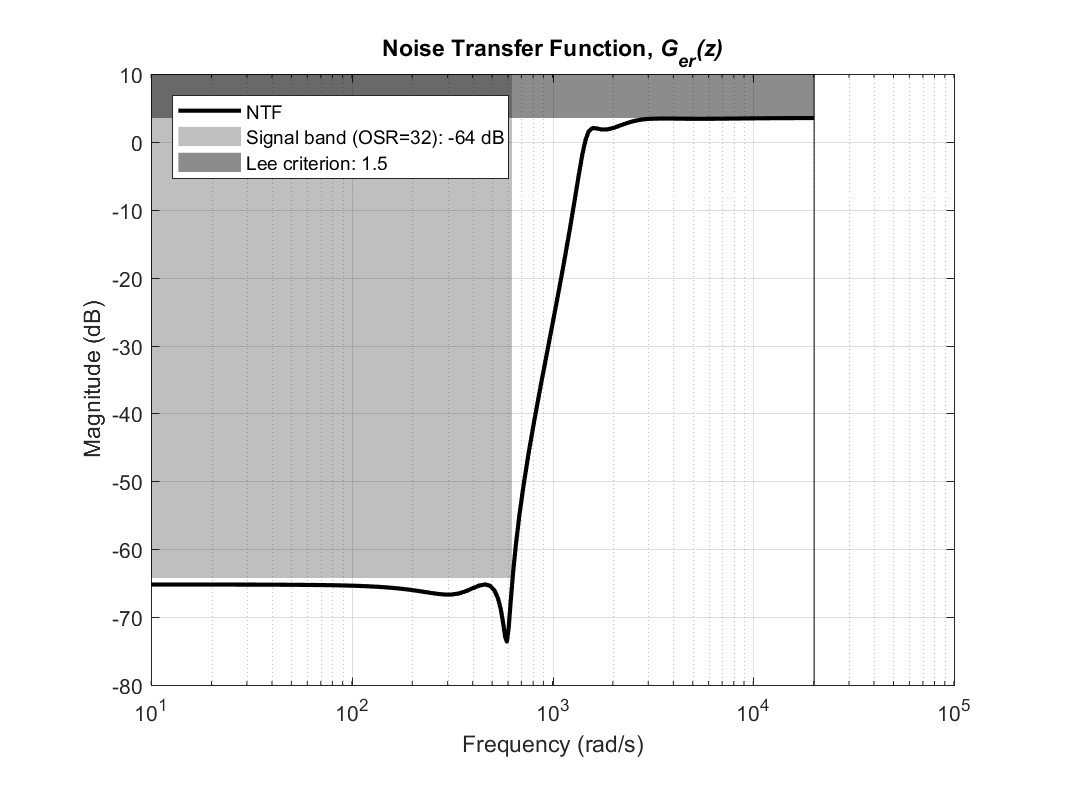
\includegraphics[width=3.45in]{ntf-hinf}
	\centering
	\caption{The sensitivity function of the design in Example~\ref{sec:ex-hinf}. The dark shaded area represents the stability constraint and the light shaded area represents the achieved noise attenuation performance.} \label{fig:ntf-hinf}
\end{figure}

\begin{figure}
	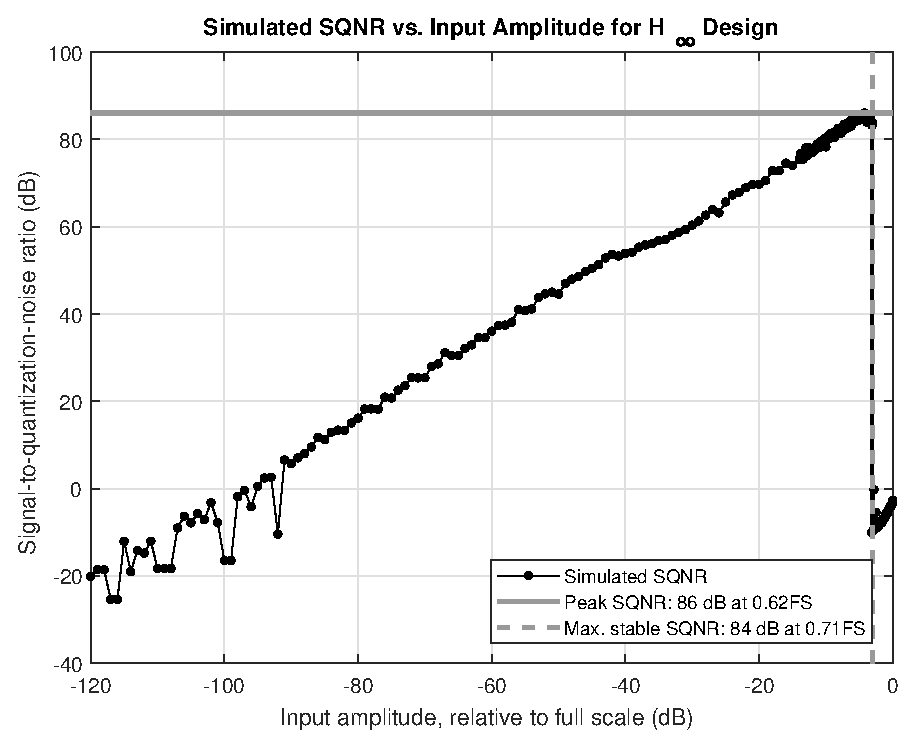
\includegraphics[width=3.45in]{sqnr-hinf}
	\centering
	\caption{An SQNR simulation with 247 points of the design in Example~\ref{sec:ex-hinf} to an input sinusoid of frequency \SI{50}{\hertz} and varying amplitude to investigate its conditional stabiilty.} \label{fig:sqnr-hinf}
\end{figure}

\begin{figure}
	\begin{NoHyper}
		\begin{center}
			\begin{tikzpicture}
				\pgfplotsset{set layers}
				\begin{axis}[
					width=3in,
					title={\textbf{Trade-off with Lee Stability Criterion}},
					scale only axis,
					xmin=1,xmax=2.2,
					ymin=50,ymax=100,
					axis y line*=left,
					xlabel={Lee criterion},
					ylabel={Maximum SQNR (dB) \ref{plt:msqnr1}},
					]
					\addplot[solid,mark=*,mark options={fill=white}] table [x=lee,y=maxSqnr,col sep=comma] {data/comparison-hinf.csv};
					\label{plt:msqnr1}
					\addplot[mark=*,mark options={fill=black}] coordinates {(1.5, 86)};
				\end{axis}
				\begin{axis}[
					width=3in,
					scale only axis,
					xmin=1,xmax=2.2,
					ymin=-50,ymax=0,
					axis y line*=right,
					axis x line=none,
					ylabel={MSIA, relative to \glsentryshort{FS} (dB) \ref{plt:msia1}},
					]
					\addplot[solid,draw=gray,mark=square*,mark options={fill=white}] table [x=lee,y=msia,col sep=comma] {data/comparison-hinf.csv};
					\label{plt:msia1}
					\addplot[mark=square*,draw=gray,mark options={fill=gray}] coordinates {(1.5, -2.975)};
					\end{axis}
			\end{tikzpicture}
		\end{center}
	\end{NoHyper}
	\caption{The performance (maximum simulated \glsentryshort{SQNR}) and stability (simulated \glsentryshort{MSIA}) achieved with the modulator design from \autoref{sec:ex-hinf} for different Lee criterion goals. The shaded markers indicate the selected design Lee criterion value.} \label{fig:lee-perf-stab}
\end{figure}

\section{Design Using Root Locus Stability Criterion}
\label{sec:ex-rl}

The root locus design technique is done by solving the \gls{GKYP} optimization problem in for performance while the constraint in \autoref{eq:rl} is enforced for robustness against the quantizer gain. Similar to the previous example, Lemma~\ref{lem:gkyp} is applied to the $r \rightarrow e$ sensitivity channel and Lemma~\ref{lem:gkyp} along with conditions in \autoref{eq:gkyp-ifi} to the $w \rightarrow z$ robustness channel. While a sufficient condition for stability would be that the root locus remains in the stable region for all positive quantizer gains \gls{K}, this produces a very conservative design. Instead, the quantizer gain robustness criterion can be used to enhance the stable input range of the design from \autoref{sec:ex-hinf}. Instablility in sigma delta modulators is often associated with low quantizer gains. To improve stability, the lower bound of the quantizer gain, $k_l$, may be changed and the optimization problem solved. Thus $k_l$ is a parameter that trades off performance and stability, which is shown in \autoref{fig:robust-perf-stab}. With some trial-and-error, $k_l=0.1$ results in a modulator that is full-scale stable under simulation. The solver converges to the loop transfer function:

\begin{equation*}
	H_1(z) = \frac{1.80\left(z - 0.806\right)\left(z - 0.641\right)\left(z^2 - 1.93z + 0.949\right)}{\left(z - 0.607\right)\left(z^2 - 1.94z + 0.943\right)\left(z^2 - 1.98z + 0.990\right)}.
\end{equation*}

\begin{figure}
	\begin{NoHyper}
		\begin{center}
			\begin{tikzpicture}
				\pgfplotsset{set layers}
				\begin{axis}[
					width=3in,
					title={\textbf{Trade-off with Root Locus Stability Criterion}},
					scale only axis,
					xmin=0,xmax=0.7,
					ymin=40,ymax=100,
					axis y line*=left,
					xlabel={Quantizer gain lower bound $k_l$},
					ylabel={Maximum SQNR (dB) \ref{plt:msqnr2}},
					]
					\addplot[solid,mark=*,mark options={fill=white}] table [x=kl,y=maxSqnr,col sep=comma] {data/comparison-robust.csv};
					\label{plt:msqnr2}
					\addplot[mark=*,mark options={fill=black}] coordinates {(0.1, 65.57)};
				\end{axis}
				\begin{axis}[
					width=3in,
					scale only axis,
					xmin=0,xmax=0.7,
					ymin=-80,ymax=0,
					axis y line*=right,
					axis x line=none,
					ylabel={MSIA, relative to \glsentryshort{FS} (dB) \ref{plt:msia2}},
					]
					\addplot[solid,draw=gray,mark=square*,mark options={fill=white}] table [x=kl,y=msia,col sep=comma] {data/comparison-robust.csv};
					\label{plt:msia2}
					\addplot[mark=square*,draw=gray,mark options={fill=gray}] coordinates {(0.1, 0)};
					\end{axis}
			\end{tikzpicture}
		\end{center}
	\end{NoHyper}
	\caption{The performance (maximum simulated \glsentryshort{SQNR}) and stability (simulated \glsentryshort{MSIA}) achieved with the modulator design from \autoref{sec:ex-rl} for different quantizer gain robustness goals. The shaded markers indicate the selected design $k_l$ value. The root locus is entirely within the unit circle for $k_l \leq 0.075$.} \label{fig:robust-perf-stab}
\end{figure}

The robustness and sensitivity channels are shown in Figure~\ref{fig:ntf-rl}. The \gls{Hinf} norm of the $G_{zw}(z)$ transfer function is less than 1 for all frequencies, showing that the system is stable for all norm-bounded quantizer gains in the range $\left[k_l, k_h\right] = \left[0.1, \infty\right)$. The root locus shown in Figure~\ref{fig:rl-rl} confirms that this is the case. A simulation like done previously shows that system is empirically stable for input amplitudes up to \gls{FS}. As expected when stability is increased, the empirical peak SQNR is reduced to \SI{66}{\deci\bel} with the minimum resolvable input amplitude at \SI{-52}{\deci\bel} \gls{FS}.

\begin{figure}
	\centering
	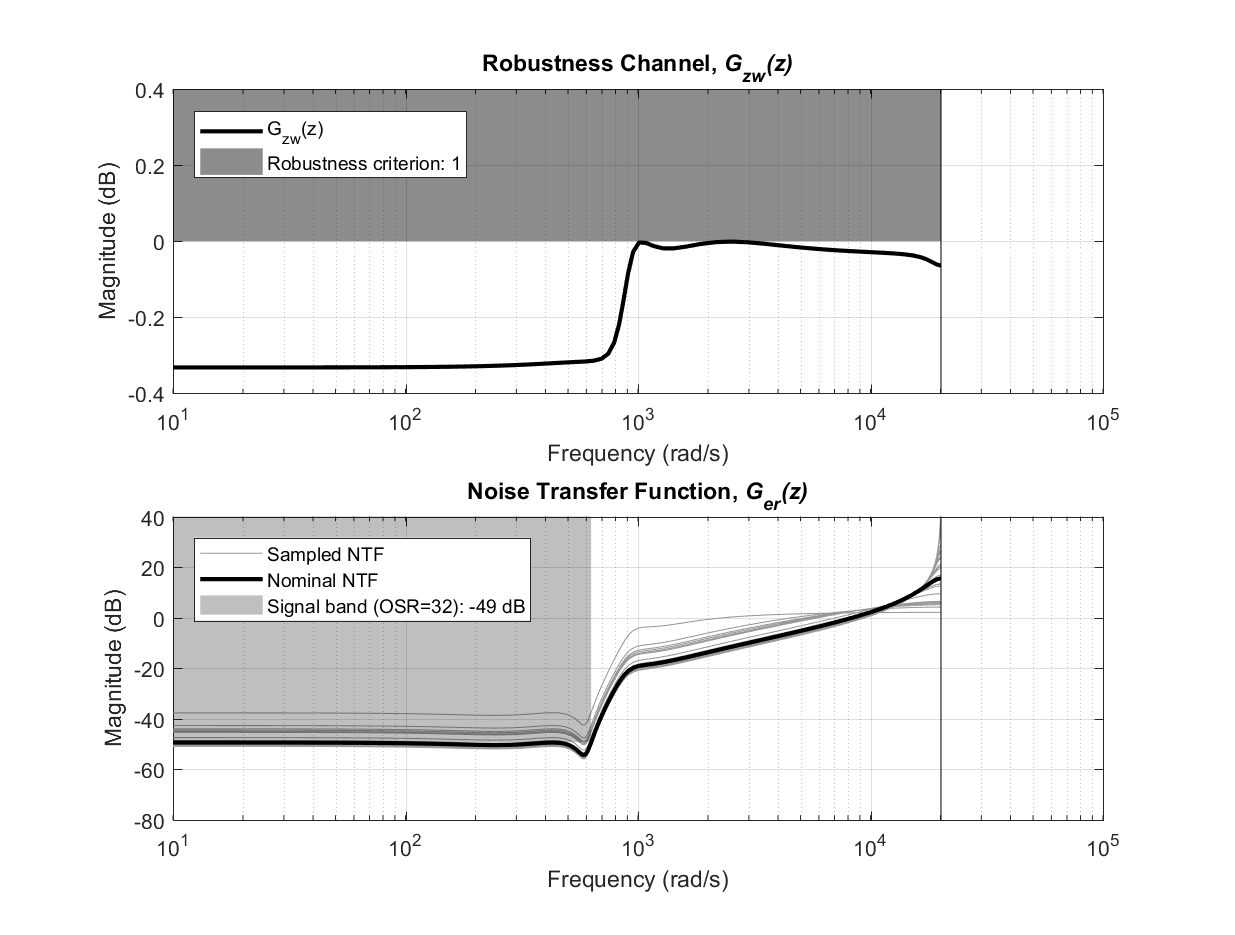
\includegraphics[width=3.45in]{ntf-robust}
	\caption{Upper: a frequency response plot of the robustness channel for the design in Example~\ref{sec:ex-rl}. Lower: the nominal sensitivity function of the same design along with sensitivity functions for randomly sampled quantizer gains with the achieved noise attenuation performance shaded.} \label{fig:ntf-rl}
\end{figure}

\begin{figure}
	\centering
	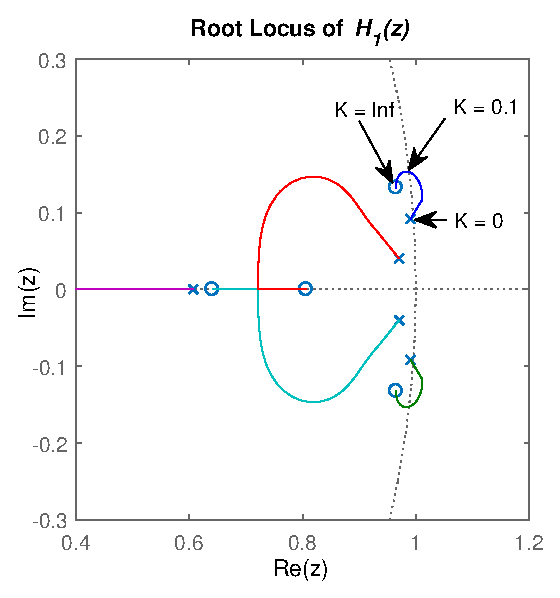
\includegraphics[width=2in]{rl-robust}
	\caption{A subset of the complex plane showing the root locus of the filter from Example~\ref{sec:ex-rl} across quantizer gains.} \label{fig:rl-rl}
\end{figure}

\section{Design Using \gls{H2} Stability Criterion}
\label{sec:ex-h2}

The \gls{H2} design technique is done by again solving the optimization problem in \autoref{eq:perf} for performance while maintaining the stability constraint from \autoref{eq:h2}. The former uses Lemma~\ref{lem:gkyp} while the latter uses Theorem~\ref{thm:h2}. In this example, the goal is to design a modulator for the same specifications as that from \autoref{sec:ex-hinf} but with slightly increased stability. One advantage of the \gls{H2} criterion is that there is a more systematic way to target a specific \gls{MSIA}. For this example, the quantizer input signal is modelled with the Gaussian \gls{PDF}. For a target \gls{MSIA} of 0.68, the criterion is satisfied if $||G_{er}(z)||^2_2<1.79$. Using this constraint along with the performance optimization, the solver converges. Even after many iterations, the \gls{LF} contains a pole-zero near cancellation indicating that the optimization scheme was not able to find a feasible 5th-order design. After simplification, the 4th-order \gls{LF} transfer function is:

\begin{equation*}
	H_1(z) = \frac{0.599\left(z - 0.654\right)\left(z^2 - 1.93z + 0.966\right)}{\left(z^2 - 1.97z + 0.972\right)\left(z^2 - 1.99z + 0.995\right)}.
\end{equation*}

Computing the NTF gain using the scale invariance procedure from \autoref{sec:stab-si}, an optimum value of $K = 0.877$ is obtained and the \gls{H2} criterion predicts stability for input signals less than 0.69 \gls{FS}. Because this stability criteria is only an approximation, the empirical \gls{MSIA} is 0.78. The peak SQNR was found to be \SI{80}{\deci\bel} at an input amplitude of 0.73. The minimum resolvable input amplitude was found to be \SI{-84}{\deci\bel} \gls{FS}. The \gls{SQNR} versus input amplitude measurements can be seen in \autoref{fig:sqnr-h2} and the trade-off between performance and stability as the \gls{H2} target is swept is shown in \autoref{fig:h2-perf-stab}.

\begin{figure}
	\centering
	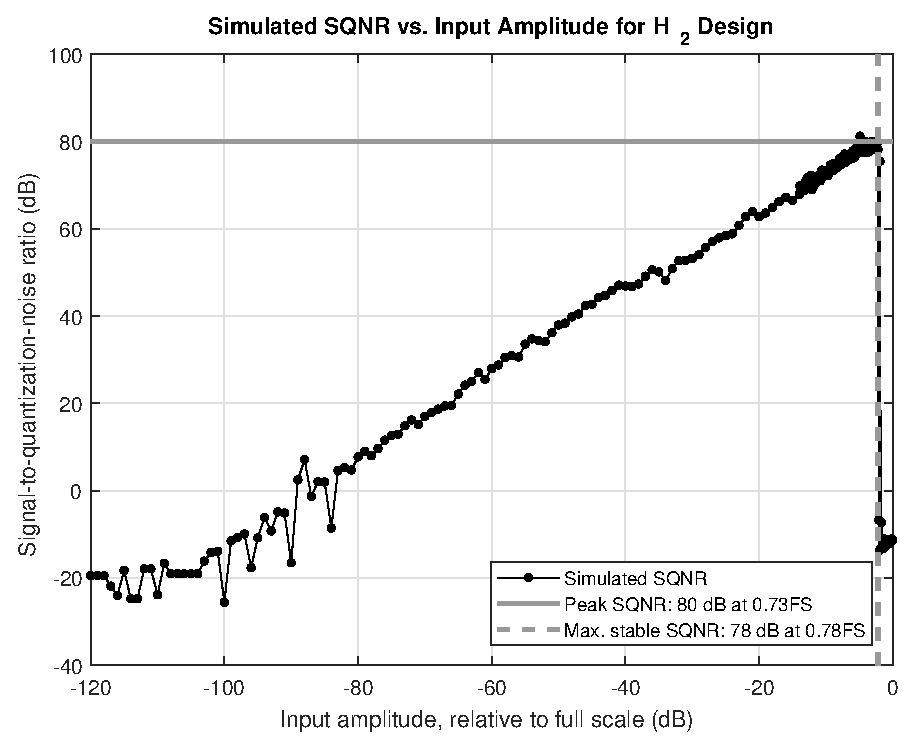
\includegraphics[width=3.45in]{sqnr-h2}
	\caption{An SQNR simulation with 247 points of the design in Example~\ref{sec:ex-h2} to an input sinusoid of frequency \SI{50}{\hertz} and varying amplitude to investigate its conditional stabiilty.} \label{fig:sqnr-h2}
\end{figure}

\begin{figure}
	\begin{NoHyper}
		\begin{center}
			\begin{tikzpicture}
				\pgfplotsset{set layers}
				\begin{axis}[
					width=3in,
					title={\textbf{Trade-off with \gls{H2} Stability Criterion}},
					scale only axis,
					xmin=1,xmax=2.8,
					ymin=60,ymax=100,
					axis y line*=left,
					xlabel={$||G_{er}(z)||_2^2$},
					ylabel={Maximum SQNR (dB) \ref{plt:msqnr3}},
					]
					\addplot[solid,mark=*,mark options={fill=white}] table [x=h22,y=maxSqnr,col sep=comma] {data/comparison-h2-2.csv};
					\label{plt:msqnr3}
					\addplot[mark=*,mark options={fill=black}] coordinates {(1.7872483786618, 79.9)};
				\end{axis}
				\begin{axis}[
					width=3in,
					scale only axis,
					xmin=1,xmax=2.8,
					ymin=-14,ymax=0,
					axis y line*=right,
					axis x line=none,
					ylabel style={align=center},
					ylabel={Simulated MSIA, relative to \glsentryshort{FS} (dB) \ref{plt:msia3-1}\\ Predicted MSIA, relative to \glsentryshort{FS} (dB) \ref{plt:msia3-2}},
					]
					\addplot[solid,draw=gray,mark=square*,mark options={fill=white}] table [x=h22,y=msia,col sep=comma] {data/comparison-h2-2.csv};
					\label{plt:msia3-1}
					\addplot[solid,draw=gray,mark=triangle*,mark options={fill=white,scale=1.5}] table [x=h22,y=targetdBopt,col sep=comma] {data/comparison-h2-2.csv};
					\label{plt:msia3-2}
					\addplot[mark=square*,draw=gray,mark options={fill=gray}] coordinates {(1.7872483786618, -2.1)};
					\addplot[mark=triangle*,draw=gray,mark options={fill=gray}] coordinates {(1.7872483786618, -3.22498532140599)};
				\end{axis}
			\end{tikzpicture}
		\end{center}
	\end{NoHyper}
	\caption{The performance (maximum simulated \glsentryshort{SQNR}) and stability achieved with the modulator design from \autoref{sec:ex-rl} for \gls{H2} norm goals. The simulated \gls{MSIA} is shown along with the predicted \glsentryshort{MSIA} using the Gaussian quantizer input \glsentryshort{PDF} and scale invariance property. The shaded markers indicate the selected design $||G_{er}(z)||_2^2$ value.} \label{fig:h2-perf-stab}
\end{figure}

\section{Design Using \gls{l1} Stability Criterion}
\label{sec:ex-l1}

\section{\titlecap{\glsentrylong{CT}} Design}
\label{sec:ex-ct}

To examine how the optimization framework may be used to directly produce \gls{CT} designs, a 3rd order \gls{CT} sigma delta modulator is produced for audio applications. Due to the absence of stability criteria that may be directly applied to continuous-time designs, the following constraints are used:

\begin{gather}
	\min_{\omega \in [0, 2\pi\cdot4.41\times10^5]} ||G_{er}(j\omega)||_\infty \quad \textrm{s.t.} \label{eq:ct-con1} \\
	||G_{er}(j\omega)||_\infty \leq \SI{4}{\deci\bel} \quad \forall \omega \label{eq:ct-con2} \\
	||G_{yr}(j\omega)||_\infty \leq \SI{-10}{\deci\bel} \quad \omega \in [2\pi\cdot7.056\times10^5, \infty) \label{eq:ct-con3}
\end{gather}

The constraint in \autoref{eq:ct-con1} uses \autoref{eq:perf} to minimize the in-band noise of the sensitivity function. The constraint in \autoref{eq:ct-con2} favours stability by placing a maximum gain on the \gls{NTF}. Unlike discrete-time designs, there is no influence of the quantizer sampling frequency captured in the first two constraints. Thus, the constraint in \autoref{eq:ct-con3} is used to force high roll-off by reducing the \gls{STF} outside the signal band.

The optimization process converges on the loop filter transfer function:

\begin{equation*}
	\frac{1.11\times10^8\left(s^2 + 3.25\times10^6 + 1.178\times10^{13}\right)}{\left(s + 2.37\times10^8\right)\left(s^2 + 3.80\times10^4 + 3.94\times10^{10}\right)},
\end{equation*}

for which the sensitivity and complementary sensitivity functions are shown in \autoref{fig:ntf-ct} and the spectrum of the simulated quantizer output is shown in \autoref{fig:fft-ct}.

\begin{figure}
	\centering
	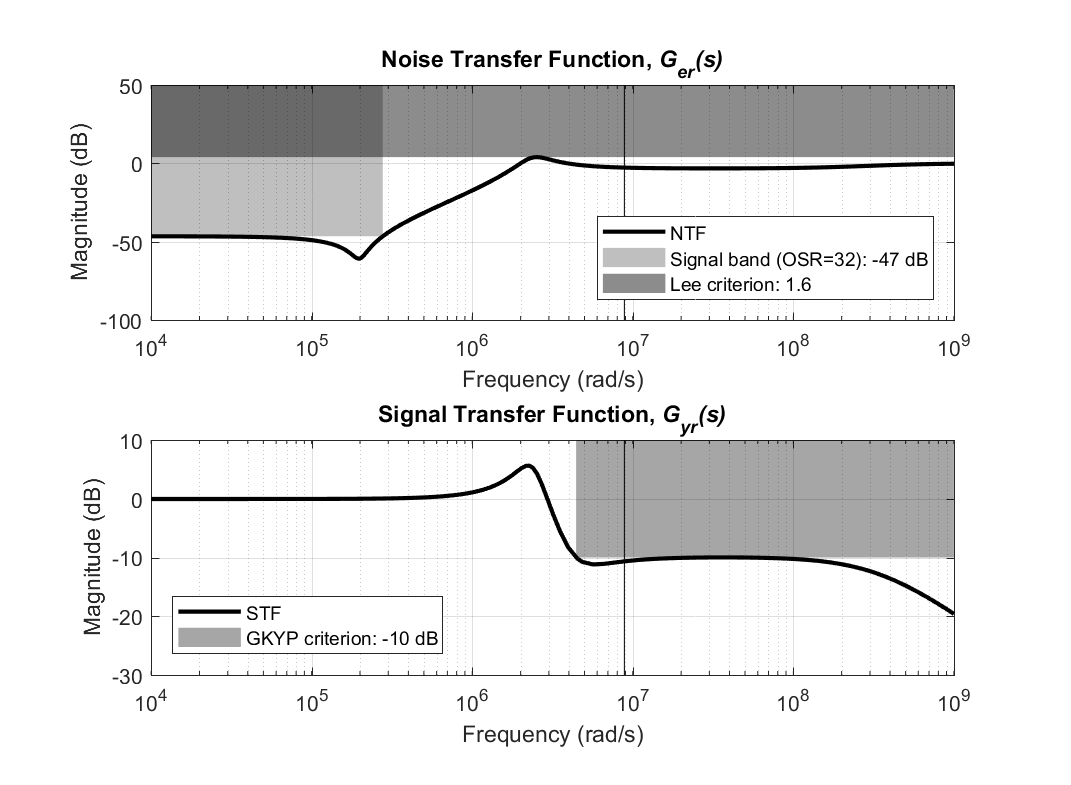
\includegraphics[width=3.45in]{ntf-ct}
	\caption{Upper: the sensitivity function of the \glsentryshort{CT} from \autoref{sec:ex-ct}. Lower: the complementary sensitivity function with a \glsentryshort{GKYP} constraint to enforce sharp roll-off.} \label{fig:ntf-ct}
\end{figure}

\begin{figure}
	\centering
	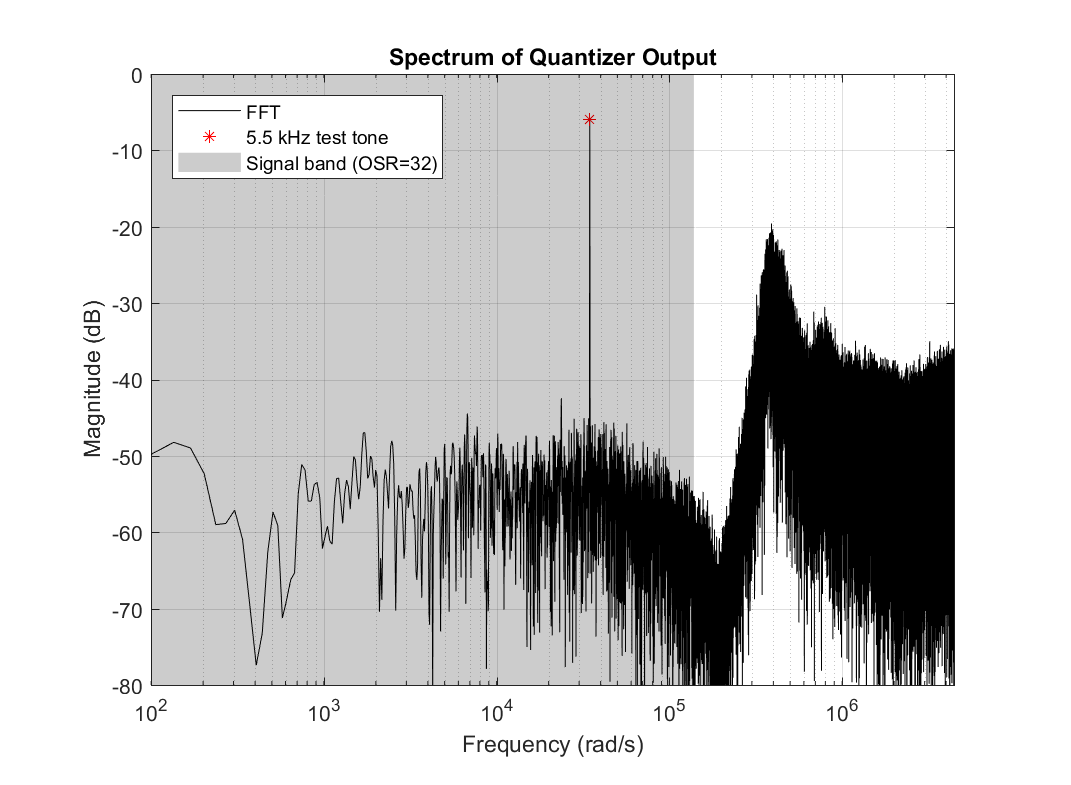
\includegraphics[width=3.45in]{fft-ct}
	\caption{The 14~000-point FFT of the quantzer output of the \glsentryshort{CT} design from Section~\ref{sec:ex-ct} shows about \SI{-40}{\deci\bel} of noise shaping to a \SI{3.46e4}{\radian\per\second} input sinsuoid with amplitude 0.5 \glsentryshort{FS}.} \label{fig:fft-ct}
\end{figure}

\section{Summary of Design Examples}
\label{sec:ex-compare}